\subsection{Experimental Setup}
\paragraph{Procedure}
\begin{enumerate}
	\item 
	\item 
	\item 
\end{enumerate}
\paragraph{Variables}
\begin{enumerate}
    \item Voltage on function generator: 10V. (control)
	\item Probes 180º from each other. Sense leads 30º from the probe; 180º from each other(control)
	\item Gain $\frac{15k}{150} = 100$ (control)
	\item liquid volume 250 ml, 60mm height measured from inside the cup(control)
	\item Frequency (independent)
	\item Voltage peak-to-peak (dependent)
\end{enumerate}

\pagebreak 
\subsection{Raw data}
\begin{figure}[h]
\begin{minipage}{0.48\textwidth}
    \centering
    \begin{tikzpicture}[scale=0.85]
	    \begin{semilogxaxis}[
	    	title={PBS solution}, xlabel=Frequency $(\si{\hertz})$, ylabel=Amplitude $(\si{\milli\volt})$, ymin=10, ymax=30, %axis x line = bottom, axis y line=left,
	    ]
	    	\addplot[] table{PBS.dat};
	    \end{semilogxaxis}
    \end{tikzpicture}
    \caption{Amplitude based on frequency. Notice the dip at \SI{50}{\hertz} due to the filter.}
    \label{fig:}
\end{minipage}
\begin{minipage}{0.48\textwidth}
	\centering
	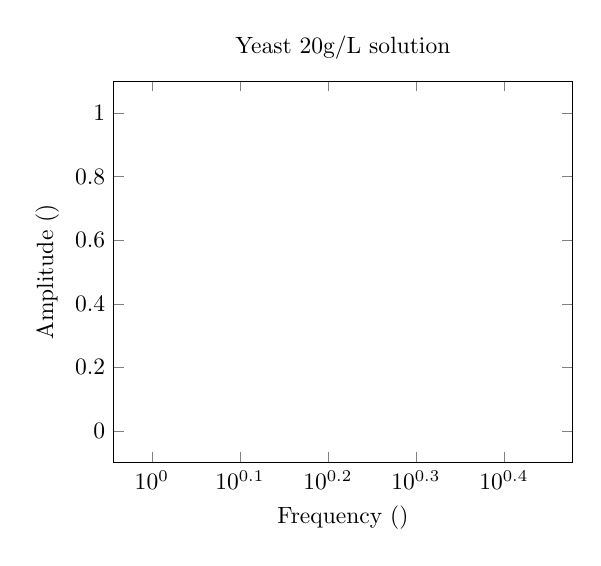
\begin{tikzpicture}[scale=0.85]
	\begin{semilogxaxis}[
	title={Yeast 20g/L solution}, xlabel=Frequency $(\si{\hertz})$, ylabel=Amplitude $(\si{\milli\volt})$
	]
%	\addplot[] table{};
	\end{semilogxaxis}
	\end{tikzpicture}
	\caption{}
	\label{}
\end{minipage}
\end{figure}

\subsection{Analysis}
PBS numbers must be compared to yeast to tell us something meaningful regarding the frequency. At the moment, there is not much we can do.